\begin{theorem}[Сидлер]
    Пусть для двух равновеликих многогранников все инварианты Дена равны, то есть для любой аддитивной функции, определённой на их двугранных углах и числе $\pi$, выполнено $f(\pi) = 0, \ f(w_1) = f(w_2) \Rightarrow w_1, w_2$ равносоставлены.
\end{theorem}

\begin{definition}
    Два равновеликих многогранника $A, B$ называются равнодополняемыми, если существуют два равносоставленных многогранника $W_A, W_B$, для которых существуют разбиения $W_A = \bigcup_{i = 1}^k P_i \cup A, \ W_B = \bigcup P_i \cup B$, где $P_i$ — многогранники.
\end{definition}

\begin{theorem}[3-я проблема Гильберта]
    Существуют ли не равнодополняемые тетраэдры с равными основаниями и высотами?
\end{theorem}

\begin{statement}
    Если многогранники $A,B$ равнодополняемые, то их инварианты Дена равны.
\end{statement}
\begin{proof}
    $f(W_A) = f(W_B)$, где $$f(W_A) = f(A) + \sum_{i = 1}^{k} f(P_i) = f(B) + \sum_{i = 1}^{k} f(P_i) = f(W_B)$$
\end{proof}

Сюда тетраэдр Хилла.

\begin{statement}
    Тетраэдр Хилла, координатный тетраэдр не равносоставлены, а также не равнодополнены.
\end{statement}

\newpage
\section{Многообразия}

\begin{definition}
    Пусть $X$ — топологическое пространство. Пусть $B$ — семейство его открытых подмножеств такое, что любое открытое множество в $X$ есть объединение множеств из $B$. $B$ называется \textit{базой топологии}.
\end{definition}

\begin{definition}
    Хаусдорфово топологическое пространство называется \textit{двумерным ($n$-мерным) многообразием}, если оно имеет счётную базу, и у любой точки существует окрестность, гомеоморфная открытому двумерному ($n$-мерному) диску.
\end{definition}

\paragraph{Классификация двумерных связных компактных многообразий}
Примеры:
\begin{enumerate}
    \item $\R^2$ — плоскость — не компактна;
    \item Сфера — связна, компактна, двумерное многообразие;
    \item Тор (см.рис.\ref{fig:thorus});
    \item Бутылка Клейна (см.рис.\ref{fig:kleyn}).
\end{enumerate}

%\clearpage
\begin{figure}[h]
    \centering
    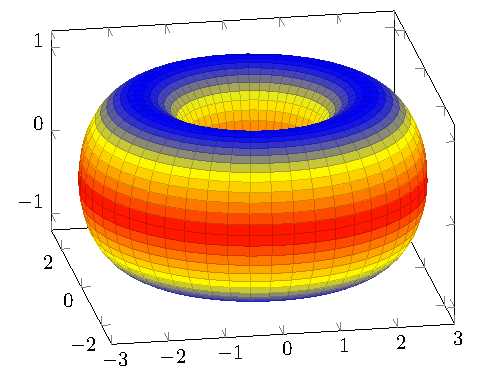
\includegraphics[scale=0.8]{images/c9.2.pdf}
    \caption{Тор}
    \label{fig:thorus}
    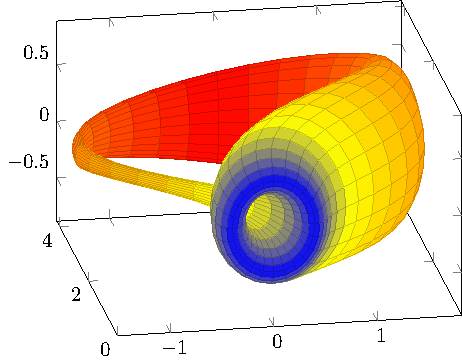
\includegraphics[scale=0.8]{images/c9.1.pdf}
    \caption{Бутылка Клейна}
    \label{fig:kleyn}
    % 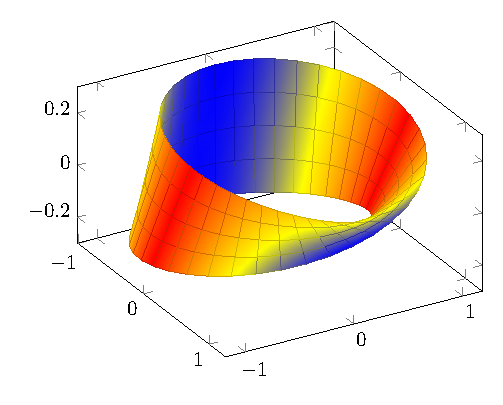
\includegraphics[scale=0.8]{images/c9.3.pdf}
    % \caption{Лента Мёбиуса}
    % \label{fig:c9.3}
\end{figure}

Существует способ описания двумерных многообразий с помощью склейки каких-то кусочков плоскости, как на рисунках \ref{fig:c9.5} и \ref{fig:c9.6}.

\begin{figure}[ht]
    \centering
    \incfig{c9.5}
    \caption{Склейка тора}
    \label{fig:c9.5}
\end{figure}

\begin{figure}[ht]
    \centering
    \incfig{c9.6}
    \caption{Склейка сферы, бутылки Клейна и проективной плоскости (слева направо)}
    \label{fig:c9.6}
\end{figure}

О том, что такое проективная плоскость ($\R \mathbb{P}^2$), читайте в следующих выпусках!

%Вроде всё, кроме девятой лекции (от 03.04.2025), здесь теперь расписано полностью. Когда доделаю лекцию, которая была в четверг — пока неясно, но выше есть хотя бы два определения оттуда. Всё, что сегодня (06.04.2025) было дописано, даже не перечитывалось, будьте осторожны!

